\documentclass{article}
\usepackage{amsmath,amssymb,setspace,verbatim,graphicx,enumerate,enumitem}
\usepackage[top=1in,bottom=1in,left=1in,right=1in,head=0.5in,foot=0.5in]{geometry}
\usepackage{caption}
\usepackage{mathtools}
% \usepackage{subcaption}
% \usepackage{subfig}
% \usepackage{subfloat}
% \usepackage{tabularx}
\usepackage{mdframed}
\usepackage{amsthm}

\newtheorem*{theorem}{Theorem}

\newenvironment{Rcode}% environment name 
{%begin code
    \begin{mdframed}
    \#R code
    \begin{small}
}
{%end code
    \end{small}
    \end{mdframed}
}

\newenvironment{console}% environment name 
{%begin code
    \begin{mdframed}
    \#Console
    \begin{small}
}
{%end code
    \end{small}
    \end{mdframed}
}

\begin{document}
\title{STDA Homework 2}
\author{Seokjun Choi}
\date{May 1, 2020}
\maketitle

\textbf{Note:}
You can get full code files at my github page: Visit https://github.com/letsjdosth/SpaTempoDA \\
See "HW2" directory.

Because I provide the full code separately, in this report 
I will show only must-necessarily key code blocks, instead of bringing the whole, verbose code.

\section{Problem 1}
\textbf{
We will carry out profile log-likelihood methods based on the provided code (HW2.R).
You may use the same simulation settings as in the provided code.
\begin{itemize}
    \item Visualize profile log-likelihood of $\rho$ for $[0.005, 0.5]$ interval.
    \item Obtain MLE for $\rho, \beta, \sigma^2$.(Hint: you may use optimize or optim function in R to get MLE of $rho$.)
\end{itemize}
}

In the given setting, We want to get the MLE from the log-likelihood function,
\[l(\beta,\sigma, \rho) \propto -\frac{1}{2} log|\Sigma(\sigma^2,\rho)| - \frac{1}{2}(Y-X\beta)'\Sigma(\sigma^2,\rho)^{-1}(Y-X\beta) \]
where $\Sigma(\sigma^2,\rho)_{i,j}= \frac{|s_i-s_j|\rho}{\sigma^2}$, the exponential covariance.
To simplify the optimization problem of the log-likelihood, I do profiling for some parameters,
$\beta$, and since exponential covariance function has good form to profile $\sigma^2$,
also for $\sigma^2$.

First of all, fix $\rho$ and calculate MLE for $\beta, \sigma^2$ analytically under the fixed $\rho$.
Then, we get
\[\hat{\beta}(\rho) = (X'\Sigma(\rho)^{-1}X)^{-1}X'\Sigma(\rho)^{-1}Y\]
\[\hat{\sigma}^2(\rho) = \frac{1}{n} (Y-X\hat{\beta}(\rho))'\Sigma(\rho)^{-1}(Y-X\hat{\beta}(\rho))\]
Plug them to the original log-likelihood function. Then we get the profile log-likelihood which depend only on $\rho$.
It may, however, not be complicate to optimize the likelihood analytically so that I optimize it numerically.
The result are summarized by below plot which illustrates the likelihood with respect to $\rho$ on the range $[0.005, 0.5]$
and its critical point.

\begin{figure}[!h]
    \centering
    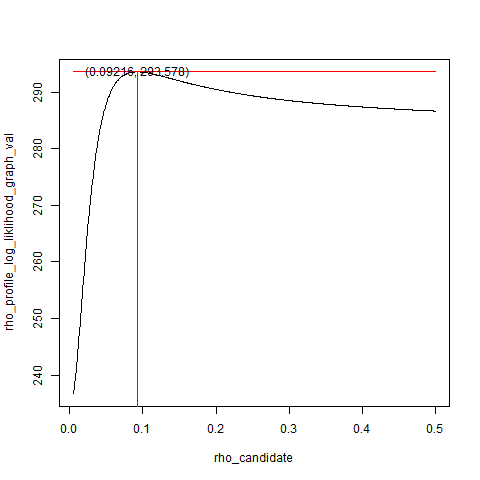
\includegraphics[height=6cm]{prob1_rho_profile_log_likelihood.png}
    \caption{the profile log-likelihood of $\rho$}
\end{figure}

The value at maximum is about $0.09216$. so
\[\hat{\rho}_{P-MLE} = 0.09216\]

Next, using this $\rho_{P-MLE}$, calculate $\hat{\beta}(\rho_{P-MLE})$ and $\hat{\sigma}^2(\rho_{P-MLE})$.
Then, we get
% write the values!
\[\hat{\beta}_{P-MLE} = 0\] 
\[\hat{\sigma}^2_{P-MLE} = 0\]
These are what we want.


\section{Problem2}
\textbf{
Following the model in page 7 of STDA4 slide, based on the provided code, do below.
\begin{itemize}
    \item Clearly write down conditional distribution for $\beta, \tau, \sigma^2, \eta_{obs}$.
        (You no need to write down for $\rho$ because there is no closed form.)
    \item Clearly write down pseudo-code of the Metropolis-Gibbs sampler.
    \item Replicate the results: (1) Provide MCMC diagnostic plots for $\beta, \tau, \sigma^2$.
        (2) Provide prediction maps (both predictive posterior mean and standard deviation).
\end{itemize}
}

Let's get conditional distributions for $\beta, \tau^2, \sigma^2, \eta_{obs}$.
For beginning, we should get a joint posterior of the parameters.
(For convenience, I deal with $\tau^2$ instead of $\tau$, and drop the 'obs' subscript of $\eta$.)

By Bayes theorem, the pdf of the joint posterior becomes
\[f(\eta,\sigma^2,\tau^2,\rho^2)\]
\[\propto f(Y|\eta,\sigma^2,\tau^2,\rho)f(\eta|\sigma^2,\tau^2,\rho)f(\sigma^2)f(\tau^2)f(\rho)\]
\[\propto N(\eta,\tau^2I) * GP(X'\beta, \sigma^2 K(\rho))
    * N(m_\beta,v_\beta) * InvGamma(a_\sigma^2, b_\sigma^2) * InvGamma(a_\tau^2, b_\tau^2)
    * Gamma(a_\rho, b_\rho) \]
\[\propto (\frac{1}{\tau^2})^n e^{-\frac{(Y-\eta)^2}{2\tau^2}}
    * (\frac{1}{(\sigma^2)^{\frac{1}{2}}})^n e^{-\frac{(\eta-X'\beta)^2}{2\sigma^2 K(\rho)}}
    * e^{-\frac{(\beta-m_\beta)^2}{2v_\beta^2}}
    * (\sigma^2)^{-a_{\sigma^2}-1} e^{-\frac{b_{\sigma^2}}{\sigma^2}}
    * (\tau^2)^{-a_{\tau^2}-1} e^{-\frac{b_{\tau^2}}{\tau^2}}
    * \rho^{a_{\rho}-1} e^{-b_{\rho}\rho}
    \]
where $K(\rho)=K(.,.,\rho)$ is exponential term of exponential covariance.

To get conditional distribution of each parameter, we just read terms of the joint distribution
including the wanted parameter. 

And note that, after mixing two gaussian kernel with respect to a parameter,
we get another normal kernel, with variance which is by inverting original two variances (or simply, 'precisions') and adding them together,
and mean which is by weighted average of original two means using precision as weights. Or,
\[e^{-\frac{(X-m_1)^2}{2v_1^2}} * e^{-\frac{(X-m2)^2}{2v_2^2}}
    \propto e^{-\frac{(X-(\frac{m_1}{v_1^2} + \frac{m_2}{v_2^2})/(\frac{1}{v_1^2} + \frac{1}{v_2^2}))^2}{2(\frac{1}{v_1^2}+\frac{1}{v_2^2})}}\]

Then, we get

for $\eta$,
\[f(\eta|\beta,\sigma^2,\tau^2,\rho,Y) \propto e^{-\frac{(\eta - (\frac{y}{\tau^2} + \frac{X'\beta}{\sigma^2 K(\rho)}) / (\frac{1}{\tau^2}+\frac{1}{\sigma^2 K(\rho)}))^2}{2(\frac{1}{\tau^2}+\frac{1}{\sigma^2 K(\rho)})}}
\]
\[\sim N(\frac{\frac{y}{\tau^2} + \frac{X'\beta}{\sigma^2 K(\rho)}}{\frac{1}{\tau^2}+\frac{1}{\sigma^2 K(\rho)}}, \frac{1}{\tau^2}+\frac{1}{\sigma^2 K(\rho)})\]

for $\beta$,
\[f(\beta|\eta,\sigma^2,\tau^2,\rho,Y) \propto e^{-\frac{(\beta - (\frac{X\eta}{\sigma^2 K(\rho)} + \frac{m_\beta}{v_\beta}) / (\frac{X^2}{\sigma^2 K(\rho)}+\frac{1}{v_\beta})^2}{2(\frac{X^2}{\sigma^2 K(\rho)}+\frac{1}{v_\beta})}}
\]
\[\sim N(\frac{\frac{X\eta}{\sigma^2 K(\rho)} + \frac{m_\beta}{v_\beta}}{\frac{X^2}{\sigma^2 K(\rho)}+\frac{1}{v_\beta}}, \frac{X^2}{\sigma^2 K(\rho)}+\frac{1}{v_\beta})\]

for $\sigma^2$,
\[f(\sigma^2|\eta,\beta,\tau^2,\rho,Y) \propto (\sigma^2)^{-(a_{\sigma^2}+\frac{n}{2})-1} e^{\frac{1}{\sigma^2}(\frac{(\eta - X'\beta)^2}{2K(\rho)}+b_{\sigma^2})}
\]
\[\sim InvGamma(a_{\sigma^2}+\frac{n}{2}, \frac{(\eta - X'\beta)^2}{2K(\rho)}+b_{\sigma^2})\]

for $\tau^2$,
\[f(\tau^2|\eta,\beta,\sigma^2,\rho,Y) \propto (\tau^2)^{-(a_{\tau^2}+\frac{n}{2})-1} e^{\frac{1}{\tau^2}(\frac{(Y - \eta)^2}{2}+b_{\tau^2})}
\]
\[\sim InvGamma(a_{\tau^2}+\frac{n}{2}, \frac{(Y - \eta)^2}{2}+b_{\tau^2})\]


Since we have conditional distributions of parameters except $\rho$,
we are ready to generate samples of the joint posterior using Metropolis-Gibbs sampler.
Sudo code is here.
\begin{mdframed}
    \begin{small}
        \begin{verbatim}
Y = data
(eta[0], beta[0], sigma_sq[0], tau_sq[0], rho[0]) = initial_values
for i in 1:sample_num:
    new_eta = random_sample_from_eta's_conditional_posterior(beta[i-1], sigma_sq[i-1], tau_sq[i-1], rho[i-1], Y)
    new_beta = random_sample_from_beta's_conditional_posterior(new_eta, sigma_sq[i-1], tau_sq[i-1], rho[i-1], Y)
    new_sigma_sq = random_sample_from_sigma_sq's_conditional_posterior(new_eta, new_beta, tau_sq[i-1], rho[i-1], Y)
    new_tau_sq = random_sample_from_tau_sq's_conditional_posterior(new_eta, new_beta, new_sigma_sq, rho[i-1], Y)
    (eta[i],beta[i],sigma_sq[i],tau_sq[i]) = new_eta, new_beta, new_sigma_sq, new_tau_sq

    proposed_rho = proposal_distribution_of_rho(rho[i-1])
    MH_ratio = non_normalized_joint_posterior(proposed_rho)*proposal_pdf(rho[i-1] | proposed_rho) / 
        (non_normalized_joint_posterior(rho[i-1])*proposal_pdf(proposed_rho | rho[i-1]))
    unif_random = random_sample_from_uniform(0,1)
    if MH_ratio > unif_random:
        rho[i] = proposed_rho
    else:
        rho[i] = rho[i-1]

Do:
    diagnostics (get traceplot, acf plot, acc-rate of rho, ESS and so on.)
    If needed, cut burn-in period and do thinning.
        \end{verbatim}
    \end{small}
\end{mdframed}

Just running the given "STDA4.R", we can replicate the posterior samples of our model.
Here are the diagnostic plots.

\clearpage
\begin{figure}[!h]
    \centering
    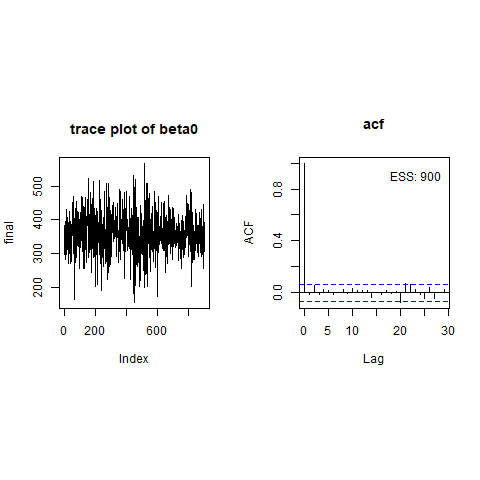
\includegraphics[height=5cm]{prob2_beta0.png}
    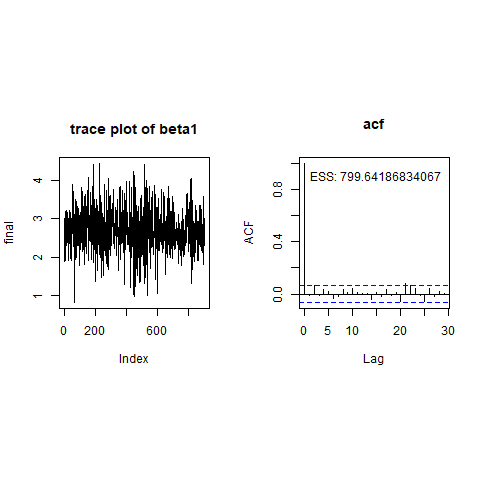
\includegraphics[height=5cm]{prob2_beta1.png} \\
    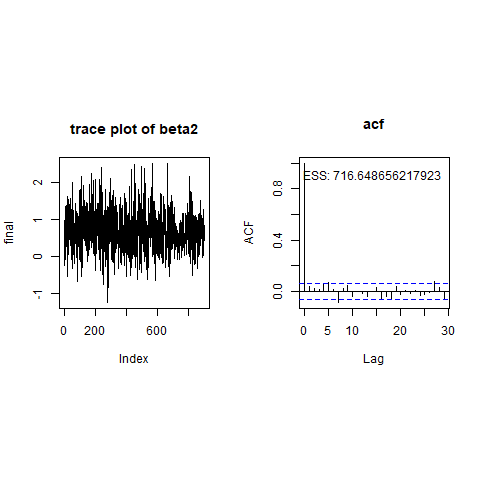
\includegraphics[height=5cm]{prob2_beta2.png}
    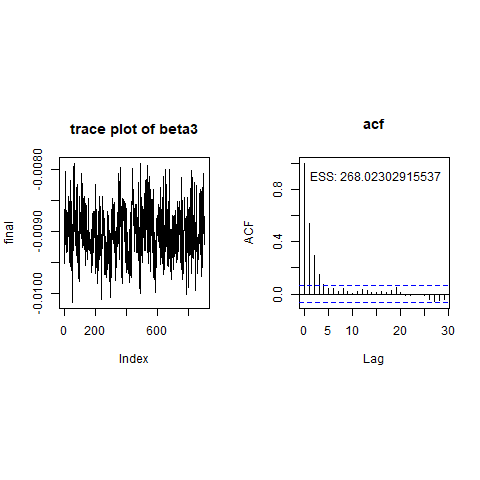
\includegraphics[height=5cm]{prob2_beta3.png} \\
    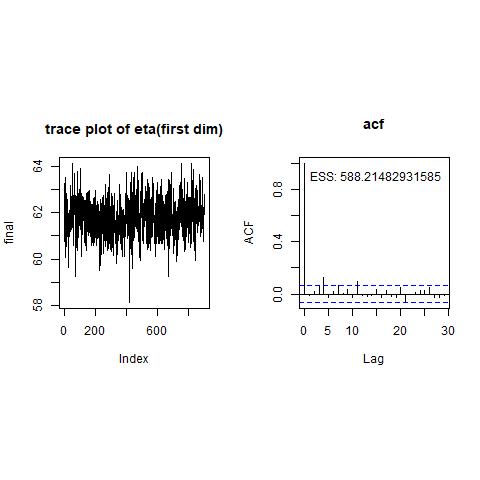
\includegraphics[height=5cm]{prob2_eta(first_dim).png}
    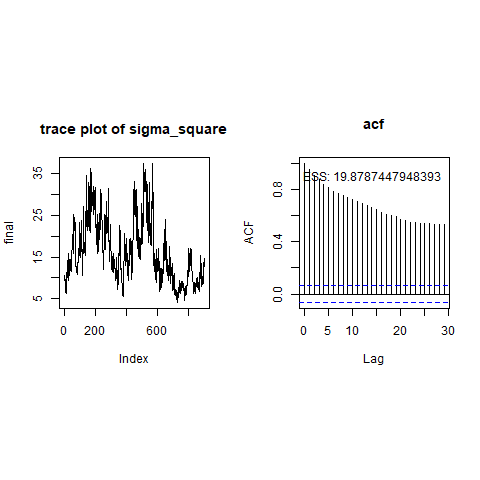
\includegraphics[height=5cm]{prob2_sigma_square.png} \\
    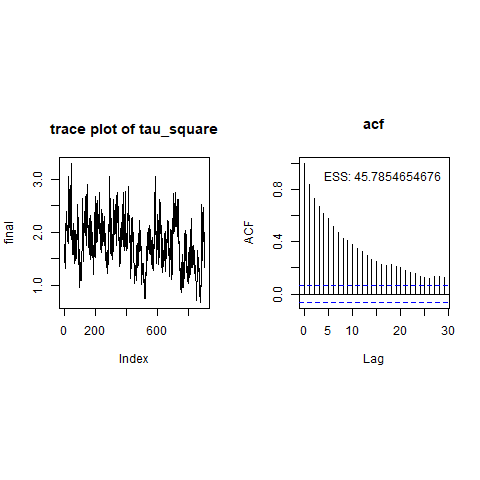
\includegraphics[height=5cm]{prob2_tau_square.png}
    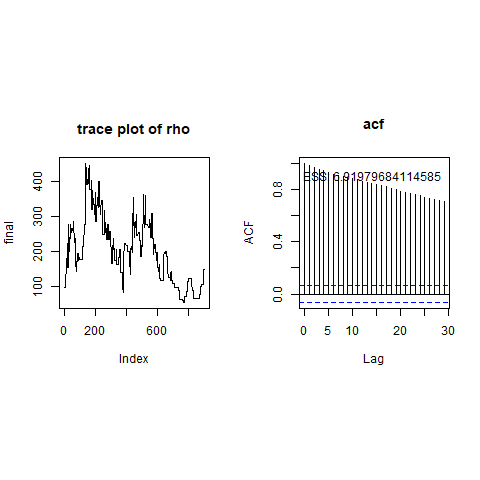
\includegraphics[height=5cm]{prob2_rho.png}
    \caption{For each parameter, left:trace-plot and ESS, right:acf plot}
\end{figure}
\clearpage

It seems that the variance-related parameters are not mixed well. 
For better inference, we had better to run longer, cut burn- in period and do thinning.
But I stop here and report raw result of Metropolis-Gibbs sampler.

Finally, here are the prediction and SE plot.


\begin{figure}[!h]
    \centering
    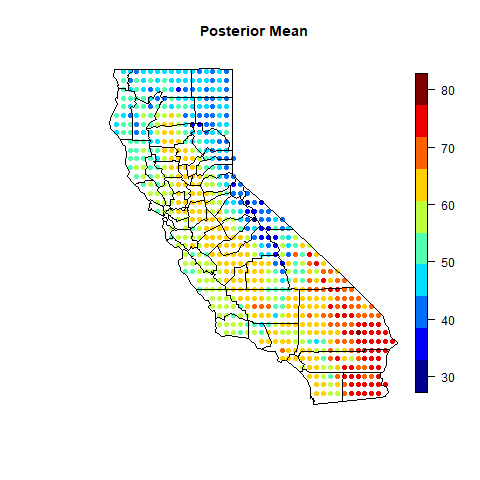
\includegraphics[height=7cm]{prob2_posterior.png}
    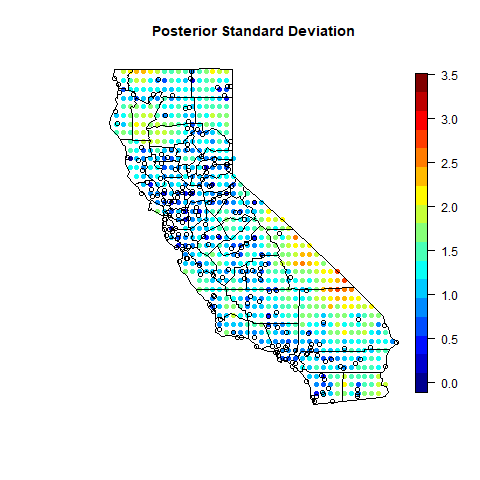
\includegraphics[height=7cm]{prob2_posterior_SE.png}
    \caption{left: prediction mean of temperature, right: standard error}
\end{figure}

Comparing these results with those of HW1, temperature values predicted by each models
are different but quite similar, and both are reasonable because the results are matched 
our common sense that the temperature are inversely related to elevation, 
and higher as go south-east in CA region.
And Standard error also fit to the expectation, which is higher in sparse data region than
dense data region.
Thus we conclude that the algorithm works well.


\end{document}